
\subsubsection{Evaluator 4 inspection scores}

\begingroup
\setlength{\tabcolsep}{1.5cm}
\renewcommand{\arraystretch}{1.45}

\rowcolors{2}{lightgray}{lightblue}
\begin{longtable}{l r}
	
	\hiderowcolors
	\textbf{Heuristic} & \textbf{Score} \\ \hline  \endhead \\
	\showrowcolors

	H1. Visibility of system status & 2  \\
	H2. Match between system and the real world & 4  \\
	H3. User control and freedom & 4 \\
	H4. Consistency and standards & 2 \\
	H5. Error prevention & 3 \\
	H6. Recognition rather than recall & 3 \\
	H7. Flexibility and efficiency of use & 3 \\
	H8. Aesthetic and minimalist design & 2 \\
	H9. Help users recognize, diagnose and recover from errors & 3 \\
	H10. Help and documentation & 3 \\
	H11. Information overload & 2 \\
	H12. Consistency of page content structure  & 2 \\
	H13. Contextualized information & 2 \\
	H14. Content organisation (hierarchy) & 4 \\
	H15. Interaction consistency & 1 \\
	H16. Group navigation-1 & 2 \\
	H17. Group navigation-2 & 3 \\
	H18. Structural navigation & 3 \\
	H19. Semantic navigation & 4 \\
	H20. “Landmarks” & 3 \\
	H21. Text lay out & 3 \\
	H22. Interaction placeholders-semiotics & 4 \\
	H23. Interaction placeholders-consistency & 1 \\
	H24. Consistency of visual elements & 3 \\
	H25. Hierarchy-1 & 3 \\
	H26. Hierarchy-2 & 3 \\
	H27. Spatial allocation-1 & 4 \\
	H28. Spatial allocation-2 & 4 \\
	H29. Consistency of page spatial structure & 2 \\
	
\end{longtable}
\endgroup

\clearpage

\subsection*{Evaluator's comments}
\paragraph*{H1. Visibility of system status – Score 2}
It's very difficult for a user to orient himself on the website, as:
\begin{itemize}
	\item Some pages show the breadcrumbs on the top left corner, while others don't.
	\item Some links on the main page lead to sub-pages that block the user from going back to the global UNICEF website. Indeed the landmark to go back to UNICEF global is very difficult to spot in these sub-pages.
\end{itemize}
Another interesting example of disorientation is when applying for a job through the website, at \href{https://jobs.unicef.org/en-us/listing/}{this link}. Once a job offer is clicked the form to be filled in doesn't report any information on the context (i.e. the job for which the application is made, the period of interest...).

\paragraph*{H2. Match between system and the real world – Score 4}
The majority of the content in the website is a description of UNICEF's missions, stories, achievements, which are all topics quite understandable from the user perspective. 
The full mark is not achieved because there are some errors that have been encountered by navigating in the website that might cause some confusion for a non-technical user. For instance there is a non-functioning button with the text "Join UNICEF" at \href{https://www.unicef.org/partnerships}{this link}.


\paragraph*{H3. User control and freedom – Score 4}
The good mark is achieved because of the search sections inside the website, for instance the search engine for publications and articles (with the icon of the magnifying glass in the top right corner of the main page), but also the \href{https://jobs.unicef.org/en-us/listing/}{search section for jobs}. In this parts of the website, a high degree of freedom is given to the user in order to apply filters, remove them and so on.
The full mark is not achieved because of the bad organization of the sub-pages of the website and the fact that inside these sub-pages the landmark for going back to UNICEF global is basically hidden in the top right corner, which limits the user freedom.



\paragraph*{H4. Consistency and standards  – Score 2}
There are a series of reasons for the low grading of this heuristic.
First off, the DONATE button, which offers one of the most fundamental actions that a user can take on the website has a different look on several pages across the website.
The symbols used for searching inside the website also change and are not consistent.
By focusing on the "All areas" section in the home page, it is also possible to notice the great inconsistency with which content is presented in the various pages for the different topics UNICEF is interested in. For instance:
\begin{itemize}
	\item These pages have different ways of showing the content, some of them through videos, some through drop-down sections or interactive elements...
	\item The resources and articles are organised differently in every page, also with different titles.
	
\end{itemize}

\paragraph*{H5. Error Prevention – Score 3}
Let's start from the assumption that the UNICEF website doesn't present many sections in which there is an intensive interaction with the user, in which case error-prone situations might arise. In any case, there are some parts of the website that are not correctly designed and report errors to the user instead of preventing them.
It is for instance possible to write any string in the search engine space, trying to inject some SQL code:

\begin{center}
	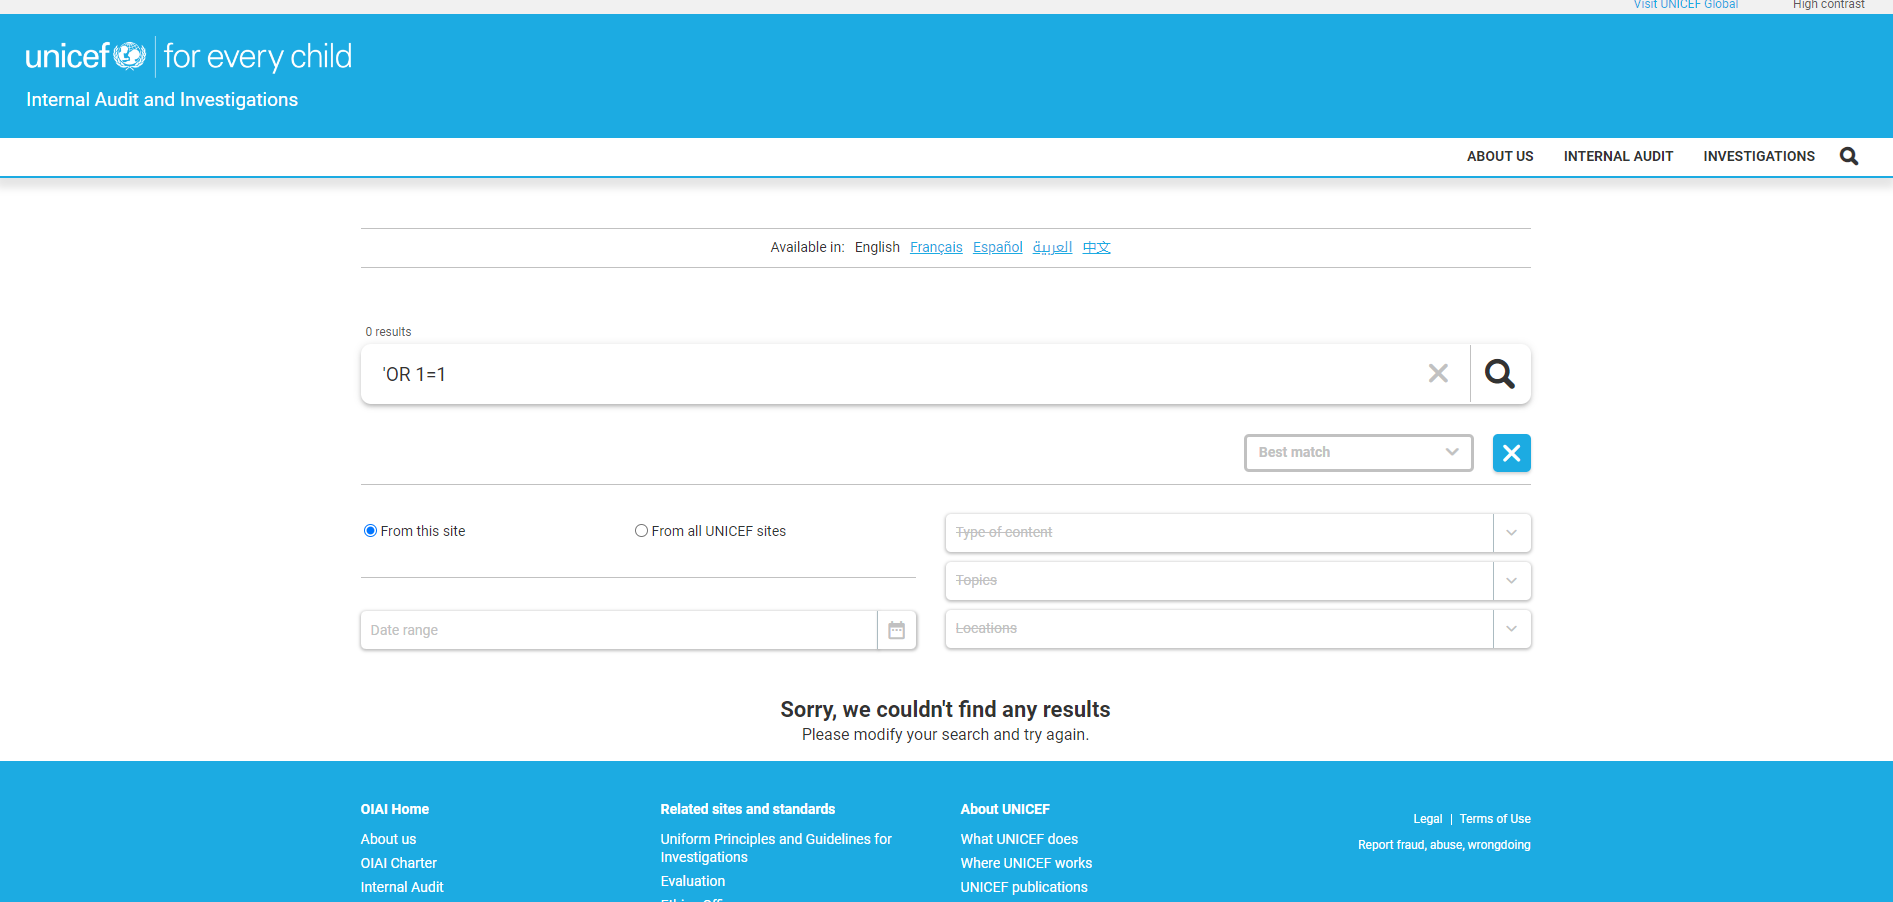
\includegraphics[width=1.1\textwidth]{\annexRes/InspectionMatteo/SQLinj}
\end{center}

\noindent
The result is the following error being displayed and not prevented:

\begin{center}
	
\includegraphics[width=1.1\textwidth]{\annexRes/InspectionMatteo/SQLinjErr}
\end{center}

Another relevant example is the page for contact under \href{https://data.unicef.org/contact/}{UNICEF Data}, where the user is asked to fill in some text fields. By trying with erroneous values (e.g. an invalid mail) no message to help the user and prevent the error is displayed. Instead, all errors show up when the "Submit" button is clicked:

\begin{center}
	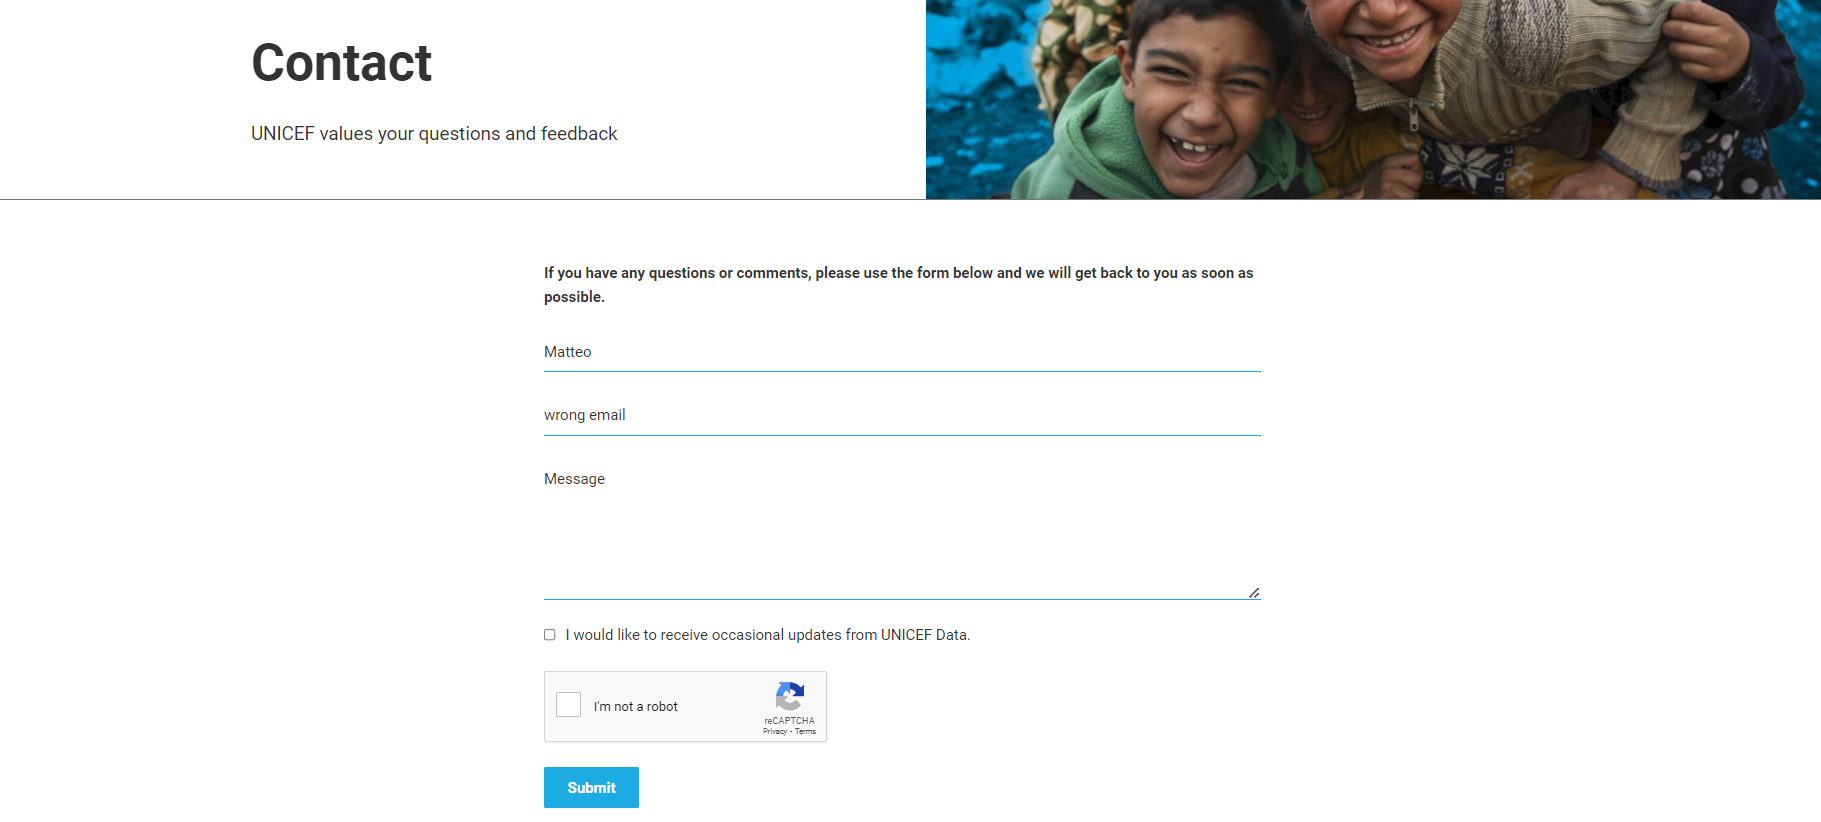
\includegraphics[width=1.1\textwidth]{\annexRes/InspectionMatteo/ContactForm}
	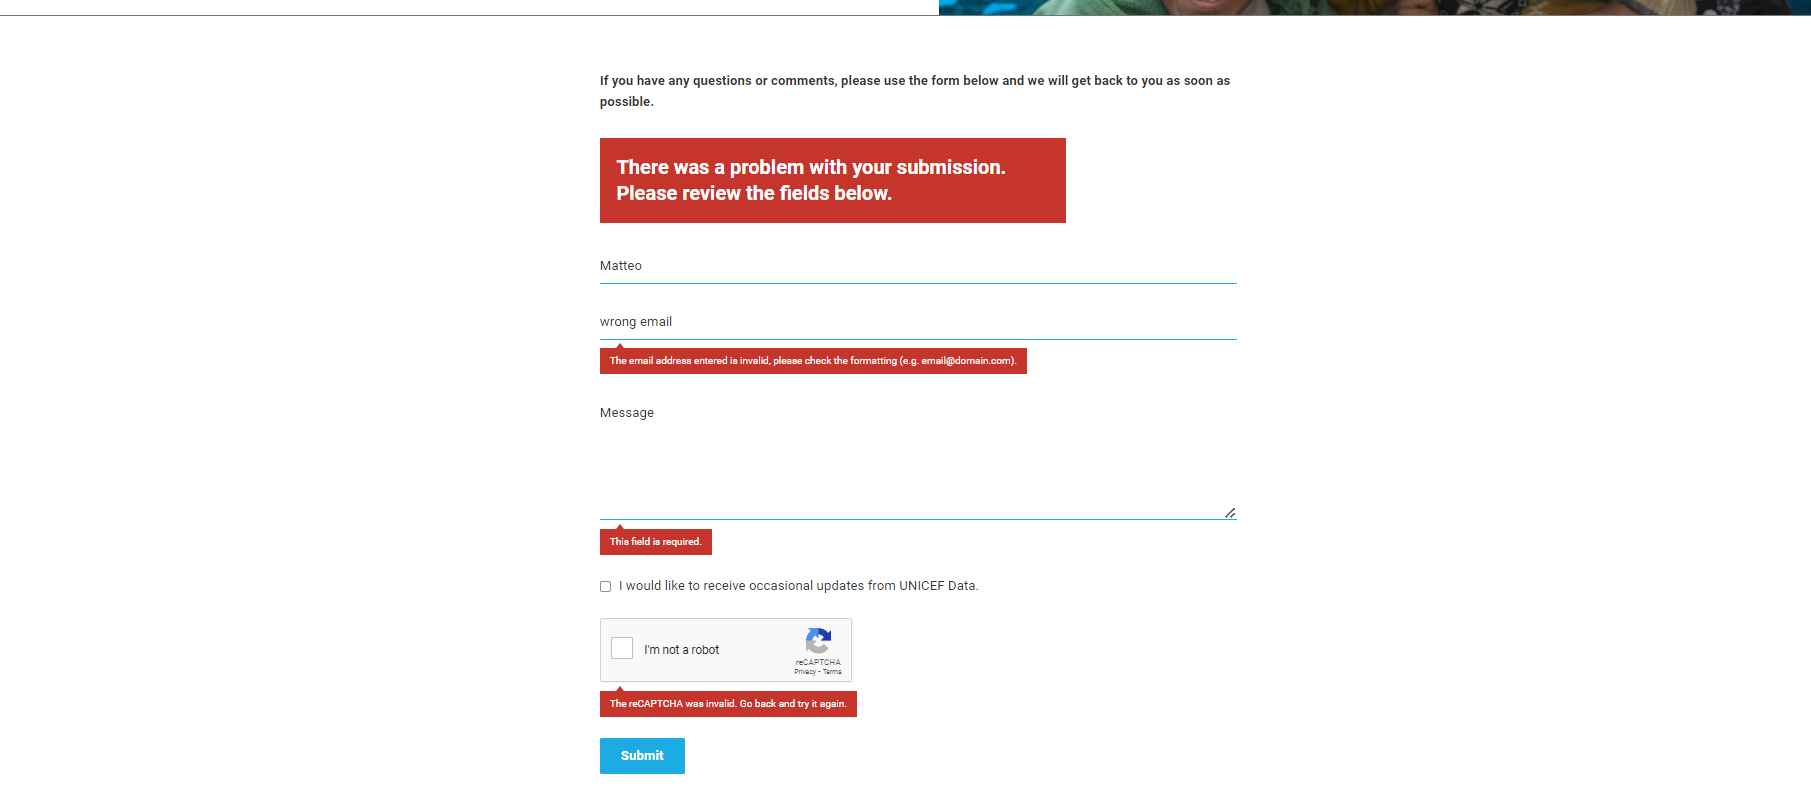
\includegraphics[width=1.1\textwidth]{\annexRes/InspectionMatteo/ContactFormErr}
	
\end{center}

\paragraph*{H6. Recognition rather than recall – Score 3}
There are some positive and some negative aspects in the overall website:
\begin{itemize}
	\item Positive: the major areas of interest for a user are highlighted thanks to the navigation bar in the home page (at the top). It is possible to choose the proper topic to focus on (there is no need to remember a specific path internal to the website).
	\item Negative: there are a lot of sub-pages whose location is not directly accessible from the home page, and in this case it is necessary to REMEMBER where to go. The most evident example is the search process for an article or a publication. There is no real internal organization of this type of content so the user doesn't have a pre-defined a guided path to reach articles s/he's interested in.
\end{itemize}


\paragraph*{H7. Flexibility and Efficiency of use – Score 3}
The website is not too bad for \textbf{efficiency} meaning that the most relevant landmarks are on the page:
\begin{itemize}
	\item Home button (landmark to go back to the home page).
	\item The navigation bar to change section that follows the user while s/he's scrolling down the pages.
	\item Search boxes or search buttons are present almost in every page.
	\item Breadcrumbs are present in some cases.
	\item Possibility to change language (when applicable, sometimes not present).
	\item Possibility to change colours and contrast on the page.
	\item There is also an accelerator for sharing the content of a page that appears in the bottom right corner of the website.
\end{itemize}

The grade is three in any case because there are some flaws that should be removed. The most relevant one is the big lack of \textbf{flexibility} of the website, in the sense that the UNICEF website doesn't adapt to a specific user. For instance, it doesn't have a dedicated personal section where users are able to store articles they want to read or links to visit again. This makes it hard to spot the same content multiple times.




\paragraph*{H8. Aesthetic and minimalist design – Score 2}
The style of the website cannot really be defined minimalist, as it is very content-intensive and in some cases it leads to a big cognitive overhead for a user that is not experienced with it. A very obvious example of this point is \href{https://www.unicef.org/reports/state-worlds-children-2023#SOWC}{this page}, in which the content, the way it is presented, the variety of colours and media types are exaggerated and create confusion for someone that has never landed on this page.

\paragraph*{H9. Help users recognize, diagnose and recover from errors – Score 3}
There are some cases in which the website stops working and doesn't give any feedback to the user to show how to escape the error state. The most evident example that has been found is on the \href{https://donazioni.unicef.it/landing/2021/07/donazioni_home/#}{donation page}, which by the way should be the most controlled one in a website like UNICEF that wants to attract as many donators as possible. 
On this page, when clicking on the landmark to go back to the home page, the following error shows up, with no way of recovering from it apart from refreshing the page:

\begin{center}
	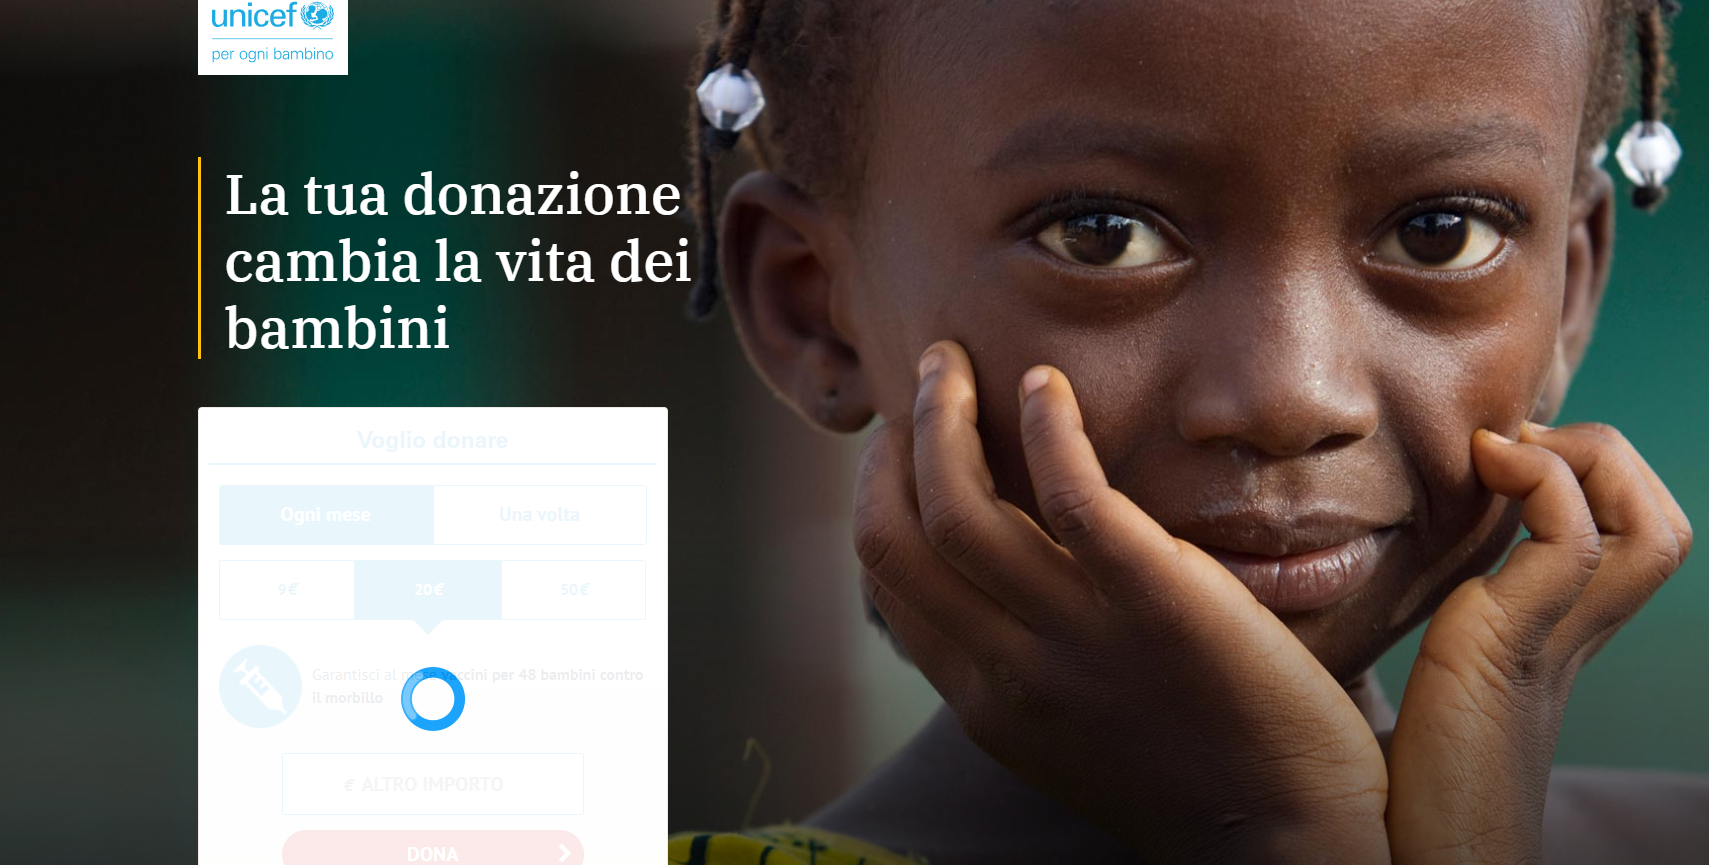
\includegraphics[width=0.9\textwidth]{\annexRes/InspectionMatteo/DonationErr}
	
\end{center}


\paragraph*{H10. Help and documentation – Score 3}
The website is quite easy to use, meaning that it doesn't require any technical background knowledge of any kind. Therefore a neutral mark is assigned.


\paragraph*{H11. Information overload – Score 2}
This heuristic might receive different evaluations based on the specific page under analysis, but overall it is fair to state that there is an exaggeration and disorganisation of the content on the UNICEF website. The most important thing that has to be mentioned here to justify the low grade is the fact that most pages under the UNICEF website are organised differently, they present the different topics using a variety of media contents (images, videos, interactive elements, colours...). This creates confusion in an inexperienced user that lands on the website for the first time and hinders the process of adaptation that should be as smooth as possible.
A clear example of information overload can be found in the presentation of the \href{https://www.unicef.org/reports/state-of-worlds-children}{\textit{The state of the world's children}} report, which is also the flagship of the agency (so it should probably be taken more care of).


\paragraph*{H12. Consistency of page content structure – Score 2}
It is possible to say that if the inspection is conducted at a very high-level, similar pages have a similar structure, but looking at the content more accurately, it's almost impossible not to spot discrepancies and different ways of structuring the same elements on the pages. 
A clear example is the case of the Resources sections for the pages \href{https://www.unicef.org/gender-equality}{Gender Equality}, \href{https://www.unicef.org/coronavirus/covid-19}{COVID-19 response} and \href{https://www.unicef.org/nutrition}{Nutrition}. The related Resources are presented in completely different ways, even if they refer to the same concept and they are also on similar pages (all the listed pages are in the same section under "What we do").

In the same way, it's very rare to find articles or blog posts with the same divisions into chapters or with the same interactions offered to the user. For instance, some articles present a donation button right in the middle of the text, while others don't.



\paragraph*{H13. Contextualized information – Score 2}
The motivations for the low grade are several:
\begin{itemize}
	\item There is no clear structure for the articles and publications, therefore the user doesn't exactly know in which point of the website s/he's located when reading.
	\item Breadcrumbs are offered very rarely and only in specific sub-pages of the website.
	\item When applying for jobs, the form to fill doesn't show any state or contextualized information to support the user in the process.
\end{itemize}


\paragraph*{H14. Content organisation  – Score 4}
The way content is displayed at a high level from the home page clearly reflects the priorities of the agency. In particular it is relevant to notice that the first section proposed for navigation is the one under "What we do", in which all the most important focus areas for UNICEF are presented and illustrated to the user.



\paragraph*{H15. Interaction consistency – Score 1}
This is probably one of the biggest flaws of the website. It is very difficult to find similar pages with the same interaction capabilities. Indeed, most of the pages have:
\begin{itemize}
	\item Different presentation of text and content: some pages have videos, some pages interactive elements for the user (maps, drop-down text sections...).
	\item Different interactions for reading the related resources. As an example, see the differences in this regard on the pages \href{https://www.unicef.org/gender-equality}{Gender Equality}, \href{https://www.unicef.org/coronavirus/covid-19}{COVID-19 response} and \href{https://www.unicef.org/nutrition}{Nutrition}.
	\item Another relevant point here is the donate button, which is important to be mentioned as it represents one of the main objectives of the website (attract donators). The donate button is interleaved with the text in some pages, while in others is not even present, and sometimes it also has different behaviours based on the page the user is located on. For example, the page dedicated to the \href{https://www.unicef.org/emergencies/delivering-support-afghanistans-children}{Afghanistan crisis} has a donate button that allows the user to donate specifically for supporting Afghanistan, while in other parts of the website the donate button leads to a general donation for the agency.
\end{itemize}

\paragraph*{H16. Group navigation-1  – Score 2}
The low grade is related to the fact that the website offers a way of navigating among related resources, articles and publications, but in a completely unorganised way, leading to confusion and disorientation in the user's experience. Indeed, all the pages on the website offer a section dedicated to related articles (or resources), but it is very difficult to conceive the grouping between these elements while the navigation is performed.
Moreover, groups of similar pages like the ones under the "What we do" section have no way of navigating from one to another apart from using the navigation bar on top.

	
	
\paragraph*{H17. Group navigation-2 – Score 3}
The website has to expose a lot of content as UNICEF is a very large agency working in many areas and countries. The grade is three because on one side the navigation bar is helpful to clarify the website structure and help with orientation inside the content. On the other hand, the way the navigation bar on top is organised could be improved in order to present the various sections in a more hierarchical manner and reduce in this way the cognitive overload for a user that lands on the website for the first time.

\paragraph*{H18. Structural navigation  – Score 3}
The grade is in the middle of the scale because there are some improvements that might be implemented but the navigation between an item and its sub-components is overall acceptable. More specifically, the website presents a structure in which content is divided based on the topic dealt with in that specific section. By navigating in any of the pages, it is almost always possible to access related content, articles, publications and so on. Unfortunately, there is no real organisation of this content, meaning that it's difficult to group articles in macro-categories and visualise the high-level representation the designers wanted to convey.

\paragraph*{H19. Semantic navigation – Score 4}
The high-grade is due to the fact that the reader is offered with a lot of related content in every page s/he visits. Many links are present inside the text, as well as related articles, posts, publications and so on. The full mark is not achieved because it is quite difficult to go back in the process, as the related content doesn't have a real classification (articles are just spread all over the website with no organisation...).
As a positive note for this heuristic, in the pages where the breadcrumbs are offered to the user to contextualise his/her position on the website, it is possible to navigate to related topics directly with the breadcrumbs.\\

\begin{center}
	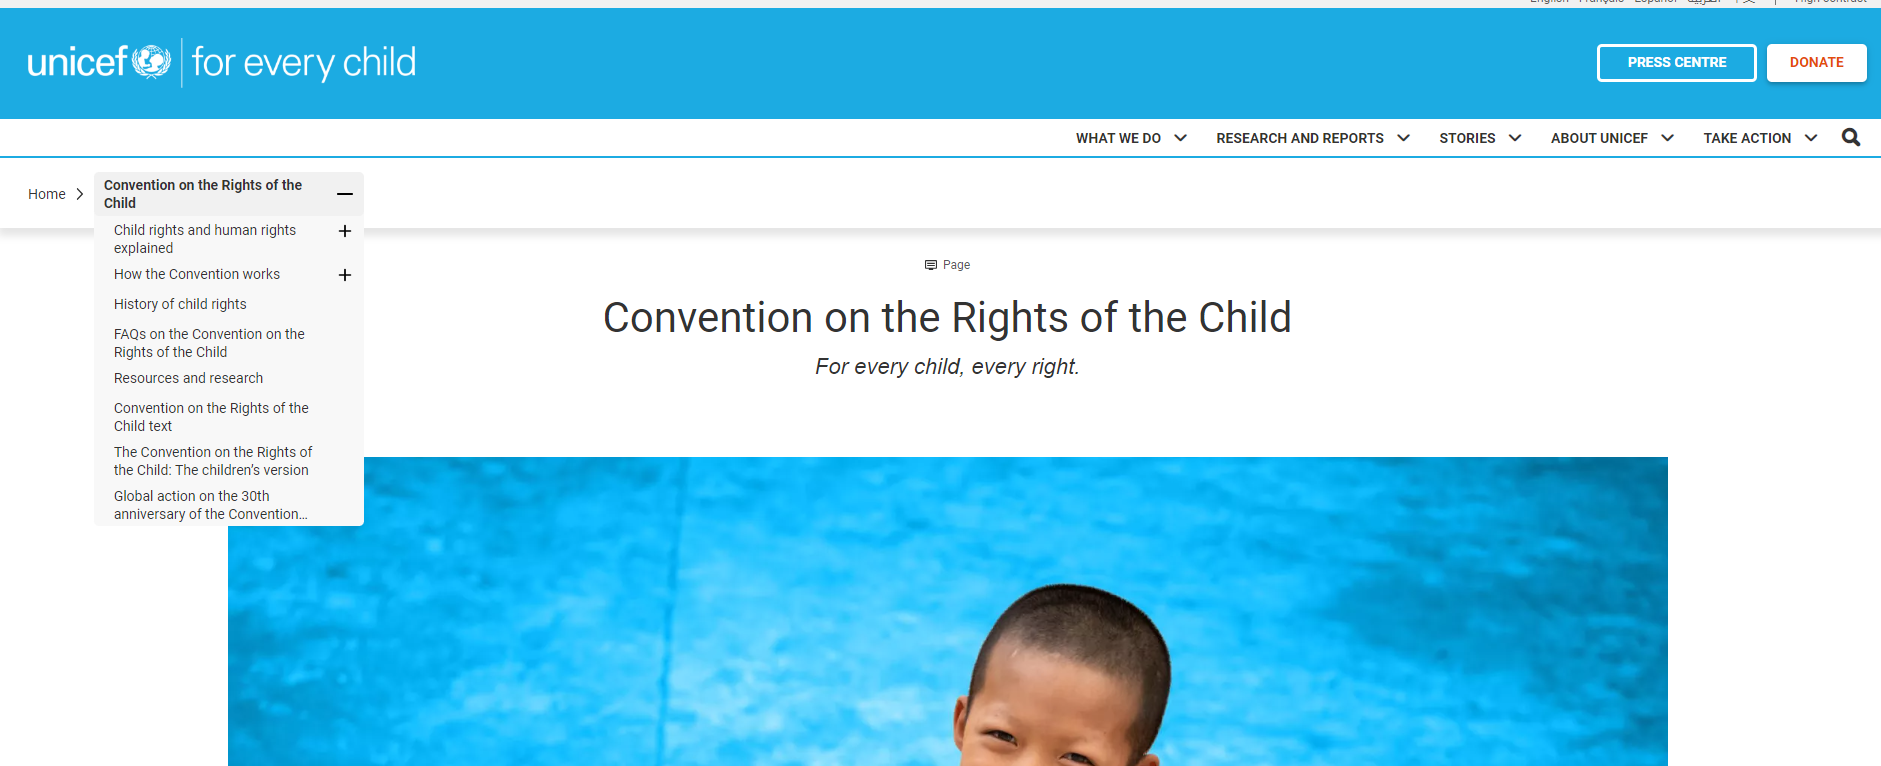
\includegraphics[width=0.9\textwidth]{\annexRes/InspectionMatteo/Breadcrumbs}
\end{center}


\paragraph*{H20. Landmarks – Score 3}
The most relevant landmarks are provided, for example the ones for going back to the home page or changing the language (since the website has to be readable by people spread all over the world). At the same time, there is space for improvement because the home page landmark changes behaviour based on the page the user is looking at. For example, every time the navigation leads to a separated sub-page of the UNICEF website, the home page landmark becomes a shortcut to that new sub-page instead of the global UNICEF website. Moreover, a new landmark is inserted to go back to UNICEF global, but it is extremely difficult to spot and it isn't given the right importance.

\begin{center}
	
\includegraphics[width=0.9\textwidth]{\annexRes/InspectionMatteo/UnicefGlobal}
\end{center}

\paragraph*{H21. Text lay out – Score 3}
The text is readable in a large portion of the website. There are some flaws that would need improvement though. For example, the text is presented in very different ways on pages that should have a similar aspect. Under the "What we do" section, in the various presentation pages for the areas of interest of the agency, the text is sometimes presented with drop-down menus, sometimes as normal text. Moreover, it should be mentioned the fact that the text is usually interleaved with images, which often times break the flow of reading and create confusion in the overall text lay out. 
Finally, the font size of the titles in the navigation bar could be increased for better readability.

\paragraph*{H22. Interaction placeholders-semiotics  – Score 4}
In the majority of cases, the meaning behind interactive elements is pretty much intuitive. The full mark is not achieved because of some specific cases encountered during the inspection. 
For example, there are some buttons under the page for \href{https://www.unicef-irc.org/}{Office of Research-Innocenti} that should increase or decrease the font size, but they don't seem so immediate to understand:
\begin{center}
	
\includegraphics[width=0.6\textwidth]{\annexRes/InspectionMatteo/Font}
\end{center}


\paragraph*{H23. Interaction placeholders-consistency – Score 1}
The low grade is due to the fact that this heuristic is rarely respected in the UNICEF website. To start with, the button for donating takes different colours and shapes throughout the application. 
In the following, some images are reported to illustrate the different ways the button is presented:

\begin{center}
	
\includegraphics[width=0.2\textwidth]{\annexRes/InspectionMatteo/Donate1}
	\hspace{2cm}
	
\includegraphics[width=0.12\textwidth]{\annexRes/InspectionMatteo/Donate2}
	\hspace{2cm}
	
\includegraphics[width=0.2\textwidth]{\annexRes/InspectionMatteo/Donate3}
\end{center}

Also the button for searching inside the website is rendered in a non uniform way, here's a couple of images to show this point:

\begin{center}
	
\includegraphics[width=0.07\textwidth]{\annexRes/InspectionMatteo/Search1} \hspace{5cm}
	
\includegraphics[width=0.3\textwidth]{\annexRes/InspectionMatteo/Search2}
\end{center}

Other examples of inconsistencies can be found for the language translation of the pages, for the links inside the text areas of the website and so on.


\paragraph*{H24. Consistency of visual elements – Score 3}
By looking at the website from a high-level point of view, it is possible to argue that there is general consistency of visual elements. For example, the majority of pages start with a title, a subtitle, and then a large image related to the topic. On the other hand, some discrepancies can be spotted if looking at the details more closely. 
For instance:
\begin{itemize}
	\item Resources have different visual representations in different pages (look at the pages \href{https://www.unicef.org/gender-equality}{Gender Equality}, \href{https://www.unicef.org/coronavirus/covid-19}{COVID-19 response} and \href{https://www.unicef.org/nutrition}{Nutrition}.)
	\item The text layout and the visual elements interleaved with text are different on similar pages.
	\item the links to jump inside text sub-sections are shown differently in different pages.
\end{itemize}

\paragraph*{H25. Hierarchy-1 – Score 3}
This heuristic is partially respected on the website. It can be noticed that all pages organize the content mostly vertically, so they don't really exploit the horizontal axis appropriately to prioritise some content over other. At the same time, a score of three is achieved since the vertical axis is often times structured correctly, having a title at the beginning, the text divided into chapters and finally related topics or resources.


\paragraph*{H26. Hierarchy-2 – Score 3}
The most relevant elements for the website are located in the top right corner, more specifically the button for donating, the options to change the language and also the navigation bar to orient in the website's content.
However, there are some flaws that show space for improvement. For instance, the search engine for articles is too little and almost hidden in the top right corner after the items belonging to the navigation bar. Moreover, when navigating to the website's sub-pages the button for going back to UNICEF global is really difficult to spot and placed in a section that doesn't reflect the importance of this landmark.
As a final note, there are some pages in which the text is interleaved with images and sometimes they're really disproportionate compared to the actual relevance they have.





\paragraph*{H27. Spatial allocation-1 – Score 4}
In most cases, this heuristic is fully respected. A clear example of this can be shown for the articles and publications that are presented in most pages of the website. They are usually very close to each other, grouped together to highlight their similarities. 

\begin{center}
	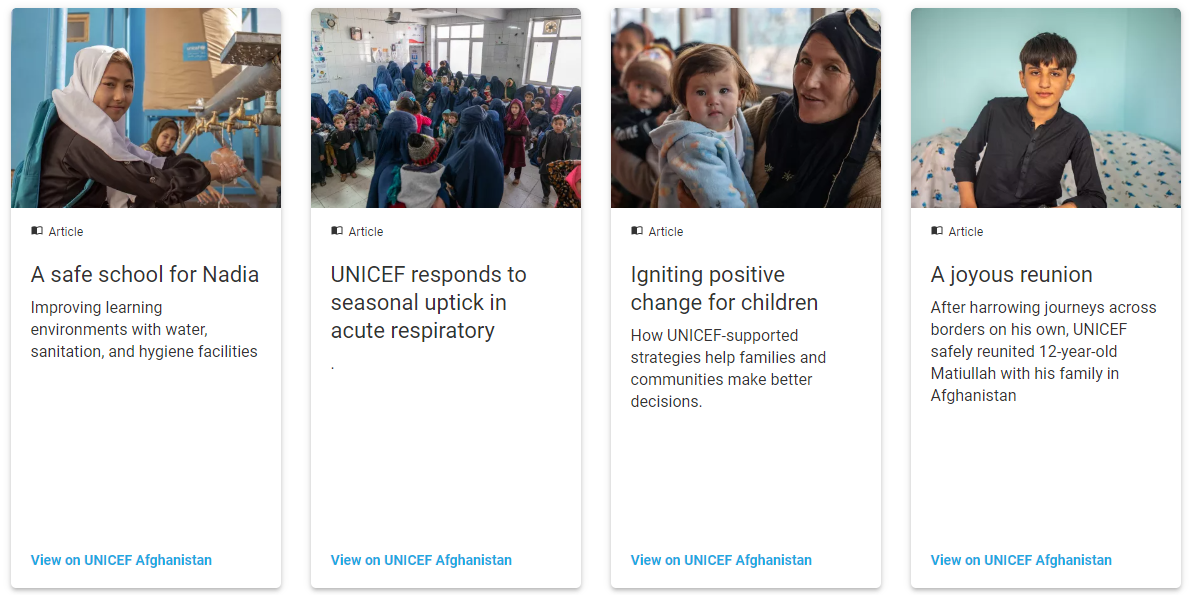
\includegraphics[width=0.9\textwidth]{\annexRes/InspectionMatteo/Articles}
\end{center}

The full mark is not achieved because there are some cases in which elements are interleaved on the page without really respecting the heuristic. An example is on the page for \href{https://www.unicef.org/reports/state-worlds-children-2023#SOWC}{\textit{The state of the world's children}} report, in which the textual description is constantly interrupted and split by other non related elements like images or other sections.


\paragraph*{H28. Spatial allocation-2  – Score 4}
This heuristic is almost fully respected throughout the website. There are rare cases in which completely unrelated elements are placed too close to each other. 
As an example, this is the visualisation of the page for \href{https://www.unicef.org/child-rights-convention}{Child Right Convention} at a very high-level (zooming out):

\begin{center}
	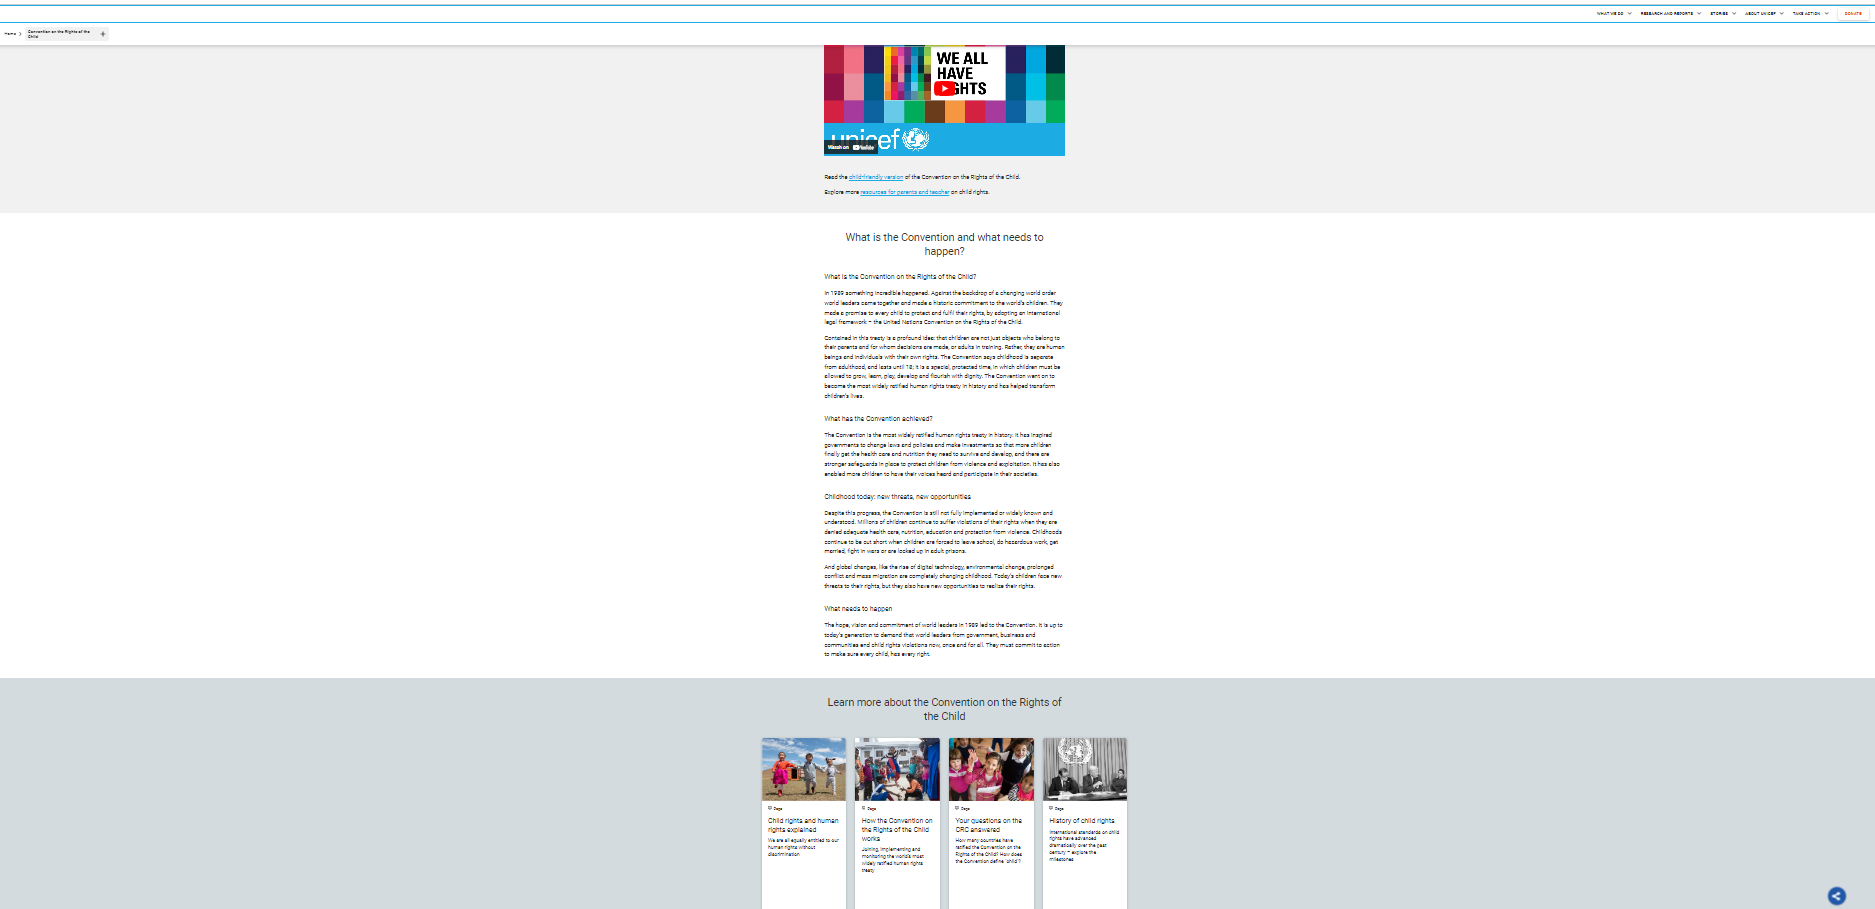
\includegraphics[width=0.9\textwidth]{\annexRes/InspectionMatteo/ChildRight}
\end{center}

It is possible to notice the division of the different parts, also supported by different colours in the background.

There are some cases in which errors emerge, if looking at the details. For example, on the page for supporting the \href{https://www.unicef.org/emergencies/delivering-support-afghanistans-children}{emergency in Afghanistan}, there are groupings of buttons with very different purposes:

\begin{center}
	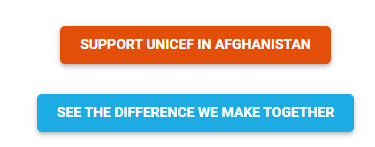
\includegraphics[width=0.5\textwidth]{\annexRes/InspectionMatteo/UnrelatedButtons}
\end{center}



\paragraph*{H29. Consistency of page spatial structure  – Score 2}
The organisation of the content really depends on the specific page. As an example, the pages under "What we do" have substantial differences in the spatial organisation of their elements. Just by looking at the three pages \href{https://www.unicef.org/gender-equality}{Gender Equality}, \href{https://www.unicef.org/coronavirus/covid-19}{COVID-19 response} and \href{https://www.unicef.org/nutrition}{Nutrition}, it is possible to notice that the resources are placed in different positions and with different layouts. The page dedicated to \href{https://www.unicef.org/gender-equality}{Gender Equality} has different sections for the resources and the latest news, while the others don't. Many other differences can be spotted on the same pages.
